\documentclass[mathserif,11pt]{beamer}

\usepackage{url,verbatim,natbib}
\usepackage[english]{babel}
\usepackage{amsmath, mathabx}
\usepackage{dsfont, ulem}
\usepackage{tikz}
\usepackage{xparse}
\newtheorem{proposition}[theorem]{Proposition}

\usepackage[headheight=22pt]{beamerthemeboxes}
\usepackage{graphicx}
\beamertemplatenavigationsymbolsempty 
\setbeamercovered{transparent}
\usepackage{centernot}

\setbeamertemplate{itemize item}{$\bullet$} 
\setbeamercolor{title}{fg=uio}
\setbeamertemplate{sections/subsections in toc}[ball unnumbered]
\setbeamercolor{section in toc}{fg=uio,bg=white}
\setbeamercolor{subsection in toc}{fg=uio,bg=white}
\setbeamercolor{result}{fg=black, bg=yellow}
\newcommand{\dotsim}{\stackrel{\cdot}{\sim}}
\newcommand{\interi}{{\rm Z}\negthinspace\negthinspace {\rm Z}}
\newcommand{\reali}{{\rm I}\negthinspace {\rm R}}
\newcommand{\naturali}{{\rm I}\negthinspace {\rm N}}
\newcommand{\sign}{\mathop{\rm sgn}\nolimits}
\newcommand{\sgn}{\mathop{\mathrm{sgn}}}
\definecolor{redve}{rgb}{0.604,0.008,0.00}
\definecolor{lmu}{rgb}{0.188,0.522,0.306}
\definecolor{uio}{rgb}{0.847,0.118,0.02}

\def\R{{\rm I\!R}}
\def\P{{\rm Pr}}
\def\Real{{\rm I\!R}}
\def\T{{\footnotesize {^{_{\sf T}}}}}
\def\tr{{\rm tr}}
\def\diag{{\rm diag}}

\NewDocumentCommand\DownArrow{O{2.0ex} O{black}}{%
   \mathrel{\tikz[baseline] \draw [<-, line width=0.5pt, #2] (0,0) -- ++(0,#1);}
}

\useframetitletemplate{% 
\begin{centering} 
\begin{small} \structure{\textcolor{uio} \insertframetitle {\insertframesubtitle}}
\end{small}

\end{centering} 
}

\addheadboxtemplate{\color[rgb]{1,1,1}}{\color{uio} \underline{{\hspace{5pt}\includegraphics[scale=0.06]{../../../../support/uio_logo_eng} \hspace{0.265\paperwidth}\color{black} \tiny  STK-IN4300 - Statistical Learning Methods in Data Science} \hspace{5pt}}}

%\bfseries{\insertsection}

\addfootboxtemplate{\color[rgb]{1,1,1}}{\color{black} \tiny \quad  
STK-IN4300: lecture 10
  \hfill \tiny \insertframenumber / \inserttotalframenumber \hspace{5pt}}

  
\title{STK-IN4300 \\ Statistical Learning Methods in Data Science}
\author{Riccardo De Bin} 
\institute{debin@math.uio.no} 
\date{}


\begin{document}
\setbeamercolor{bgr}{fg=black,bg=uio}

{
\setbeamertemplate{headline}{}
\frame{
\vspace{-2cm}
\begin{beamercolorbox}[sep=-2.2em,wd=5cm,colsep=0.5pt,ht=4.25ex,dp=3ex,left]{postit}
\includegraphics[scale=0.06]{../../../../support/uio_logo_eng}
\end{beamercolorbox}
\vspace{0.365cm}
\noindent\makebox[\linewidth]{\color{uio} \rule{\paperwidth}{0.4pt}}
\vspace{2.5cm}
\titlepage
}
}

\frame{\frametitle{Outline of the lecture}
\tableofcontents
}


\section{AdaBoost}

\subsection{Introduction}

\frame{\frametitle{AdaBoost: }
\framesubtitle{introduction}
L. Breiman: {\it ``[Boosting is] the best off-shelf classifier in the world''}.

\begin{itemize}
\item \textcolor{uio}{originally} developed for classification;
\item as a pure machine learning \textcolor{uio}{black-box};
\item \textcolor{uio}{translated} into the statistical world \citep{FriedmanAl2000};
\item extended to \textcolor{uio}{every statistical problem} \citep{MayrAl2014b},
\begin{itemize}
\item regression;
\item survival analysis;
\item \dots
\end{itemize}
\item \textcolor{uio}{interpretable} models, thanks to the statistical view;
\item extended to work in \textcolor{uio}{high-dimensional} settings \citep{Buehlmann2006}.
\end{itemize}
}


\frame{\frametitle{AdaBoost: }
\framesubtitle{introduction}
\uline{Starting challenge:}

``Can [a committee of blockheads] somehow arrive at \textcolor{uio}{highly reasoned decisions}, despite the \textcolor{uio}{weak judgement} of the individual members?'' \citep{SchapireFreund2014}

\vspace{12pt}

\uline{Goal:} create a good classifier by \textcolor{uio}{combining several weak} classifiers,
\begin{itemize}
\item in classification, a ``weak classifier'' is a classifier which is able to produce results \textcolor{uio}{only slightly better} than a random guess;
\end{itemize}

\vspace{12pt}

\uline{Idea:} apply repeatedly (\textcolor{uio}{iteratively}) a weak classifier to \textcolor{uio}{modifications of the data},
\begin{itemize}
\item at each iteration, give \textcolor{uio}{more weight} to the misclassified observations.
\end{itemize}
}


\frame{\frametitle{AdaBoost: }
\framesubtitle{introduction}
\centering
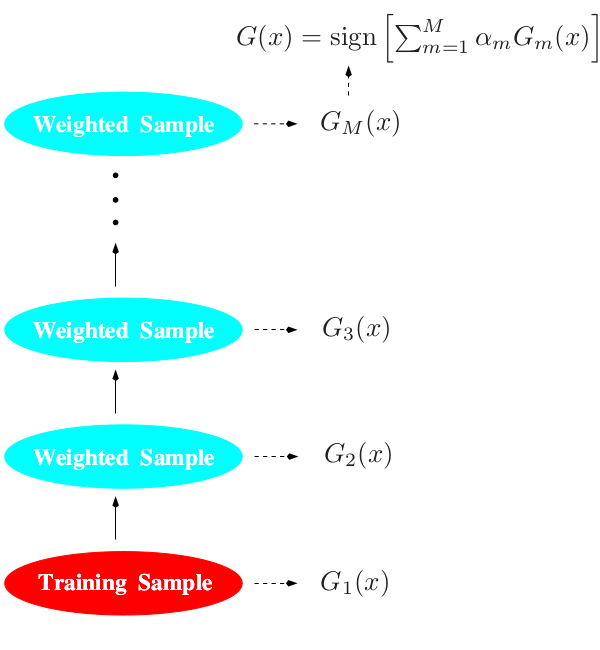
\includegraphics[width=0.68\textwidth]{fig10_1}
}



\subsection{algorithm}

\frame{\frametitle{AdaBoost: }
\framesubtitle{algorithm}
Consider a \textcolor{uio}{two-class} classification problem, $\textcolor{uio}{y_i\in\{-1,1\}}$, $x_i \in \mathds{R}^p$.

\uline{AdaBoost algorithm:}
\begin{enumerate}
\setlength\itemsep{5pt}
\item \textcolor{uio}{initialize} the weights, $w^{[0]} = (1/N, \dots, 1/N)$;
\item for $m$ from 1 to \textcolor{uio}{$m_\text{stop}$},
\begin{itemize}
\setlength\itemsep{2.5pt}
\item[(a)] \textcolor{uio}{fit the weak estimator} $G(\cdot)$ to the weighted data;
\item[(b)] compute the weighted in-sample \textcolor{uio}{missclassification rate},\\
\hspace{24pt} $\text{err}^{[m]} = \sum_{i = 1}^N w_i^{[m-1]}\mathds{1}(y_i \neq \hat{G}^{[m]}(x_i))$;
\item[(c)] compute the \textcolor{uio}{voting weights}, $\alpha^{[m]} = \log((1 - \text{err}^{[m]})/\text{err}^{[m]})$;
\item[(d)] \textcolor{uio}{update} the weights
\begin{itemize}
\item $\tilde{w}_i = w^{[m-1]}_i\exp\{\alpha^{[m]}\mathds{1}(y_i \neq \hat{G}^{[m]}(x_1))\}$;
\item $w_i^{[m]} = \tilde{w}_i/\sum_{i=1}^N \tilde{w}_i$;
\end{itemize}
\end{itemize}
\item compute the \textcolor{uio}{final result},
$$
\hat{G}_\text{AdaBoost} = \text{sign}(\sum_{m = 1}^{m_\text{stop}} \alpha^{[m]}\hat{G}^{[m]}(x_1))
$$
\end{enumerate}
}


\frame{\frametitle{AdaBoost: }
\framesubtitle{example}
\centering
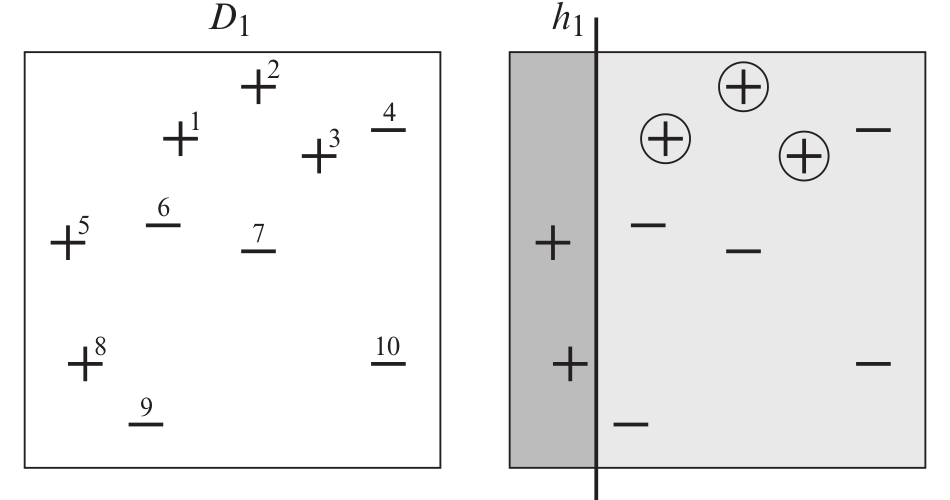
\includegraphics[width=\textwidth]{fig1_1_a}

figure from \cite{SchapireFreund2014}
}


\frame{\frametitle{AdaBoost: }
\framesubtitle{example}
{\bf First iteration:}
\begin{itemize}
\item apply the classier $G(\cdot)$ on observations with weights:
\end{itemize}
\hspace{-18pt}
\begin{tabular}{ccccccccccc}
& 1 & 2 & 3 & 4 & 5 & 6 & 7 & 8 & 9 & 10 \\
\hline
$w_i$ & $\mathbf{0.10}$ & $\mathbf{0.10}$ & $\mathbf{0.10}$ & $0.10$ & $0.10$ & $0.10$ & $0.10$ & $0.10$ & $0.10$ & $0.10$ \\
\hline
\end{tabular}

\vspace{6pt}

\begin{itemize}
\item observations 1, 2 and 3 are \textcolor{uio}{misclassified} $\Rightarrow$ err$^{[1]}=0.3$;
\item compute $\alpha^{[1]} = 0.5\log((1 - \text{err}^{[1]})/\text{err}^{[1]})\approx 0.42$;
\item set $w_i = w_i \exp\{\alpha^{[1]}\mathds{1}(y_i \neq \hat{G}^{[1]}(x_i))\}$:
\end{itemize}
\hspace{-18pt}
\begin{tabular}{ccccccccccc}
& 1 & 2 & 3 & 4 & 5 & 6 & 7 & 8 & 9 & 10 \\
\hline
$w_i$ & $0.15$ & $0.15$ & $0.15$ & $0.07$ & $0.07$ & $0.07$ & $0.07$ & $0.07$ & $0.07$ & $0.07$ \\
\hline
\end{tabular}
}



\frame{\frametitle{AdaBoost: }
\framesubtitle{example}
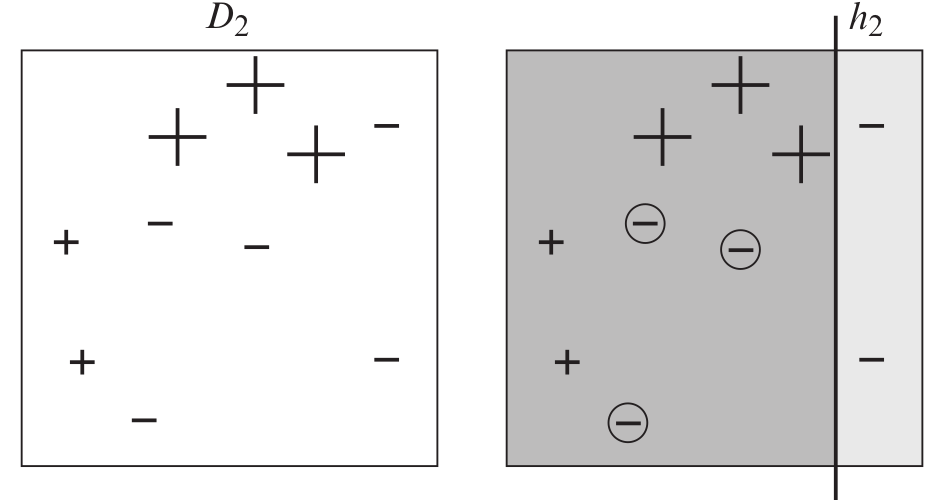
\includegraphics[width=\textwidth]{fig1_1_b}

figure from \cite{SchapireFreund2014}
}

\frame{\frametitle{AdaBoost: }
\framesubtitle{example}
{\bf Second iteration:}
\begin{itemize}
\item apply classifier $G(\cdot)$ on \textcolor{uio}{re-weighted} observations ($w_i/\sum_i w_i$):
\end{itemize}
\hspace{-18pt}
\begin{tabular}{ccccccccccc}
& 1 & 2 & 3 & 4 & 5 & 6 & 7 & 8 & 9 & 10 \\
\hline
$w_i$ & $0.17$ & $0.17$ & $0.17$ & $0.07$ & $0.07$ & $\mathbf{0.07}$ & $\mathbf{0.07}$ & $0.07$ & $\mathbf{0.07}$ & $0.07$ \\
\hline
\end{tabular}

\vspace{6pt}

\begin{itemize}
\item observations 6, 7 and 9 are \textcolor{uio}{misclassified} $\Rightarrow$ err$^{[2]}\approx0.21$;
\item compute $\alpha^{[2]} = 0.5\log((1 - \text{err}^{[2]})/\text{err}^{[2]})\approx 0.65$;
\item set $w_i = w_i \exp\{\alpha^{[2]}\mathds{1}(y_i \neq \hat{G}^{[2]}(x_i))\}$:
\end{itemize}
\hspace{-18pt}
\begin{tabular}{ccccccccccc}
& 1 & 2 & 3 & 4 & 5 & 6 & 7 & 8 & 9 & 10 \\
\hline
$w_i$ & $0.09$ & $0.09$ & $0.09$ & $0.04$ & $0.04$ & $0.14$ & $0.14$ & $0.04$ & $0.14$ & $0.04$ \\
\hline
\end{tabular}
}


\frame{\frametitle{AdaBoost: }
\framesubtitle{example}
\centering
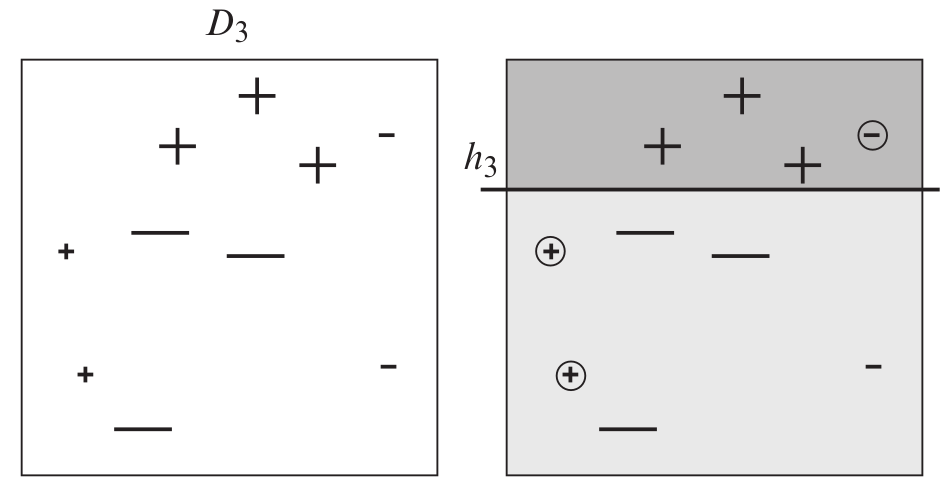
\includegraphics[width=\textwidth]{fig1_1_c}

figure from \cite{SchapireFreund2014}
}


\frame{\frametitle{AdaBoost: }
\framesubtitle{example}
{\bf Third iteration:}
\begin{itemize}
\item apply classifier $G(\cdot)$ on \textcolor{uio}{re-weighted} observations ($w_i/\sum_i w_i$):
\end{itemize}
\hspace{-18pt}
\begin{tabular}{ccccccccccc}
& 1 & 2 & 3 & 4 & 5 & 6 & 7 & 8 & 9 & 10 \\
\hline
$w_i$ & $0.11$ & $0.11$ & $0.11$ & $\mathbf{0.05}$ & $\mathbf{0.05}$ & $0.17$ & $0.17$ & $\mathbf{0.05}$ & $0.17$ & $0.05$ \\
\hline
\end{tabular}

\vspace{6pt}

\begin{itemize}
\item observations 4, 5 and 8 are \textcolor{uio}{misclassified} $\Rightarrow$ err$^{[3]}\approx0.14$;
\item compute $\alpha^{[3]} = 0.5\log((1 - \text{err}^{[3]})/\text{err}^{[3]})\approx 0.92$;
\item set $w_i = w_i \exp\{\alpha^{[3]}\mathds{1}(y_i \neq \hat{G}^{[3]}(x_i))\}$:
\end{itemize}
\hspace{-18pt}
\begin{tabular}{ccccccccccc}
& 1 & 2 & 3 & 4 & 5 & 6 & 7 & 8 & 9 & 10 \\
\hline
$w_i$ & $0.04$ & $0.04$ & $0.04$ & $0.11$ & $0.11$ & $0.07$ & $0.07$ & $0.11$ & $0.07$ & $0.02$ \\
\hline
\end{tabular}
}


\frame{\frametitle{AdaBoost: }
\framesubtitle{example}
\centering
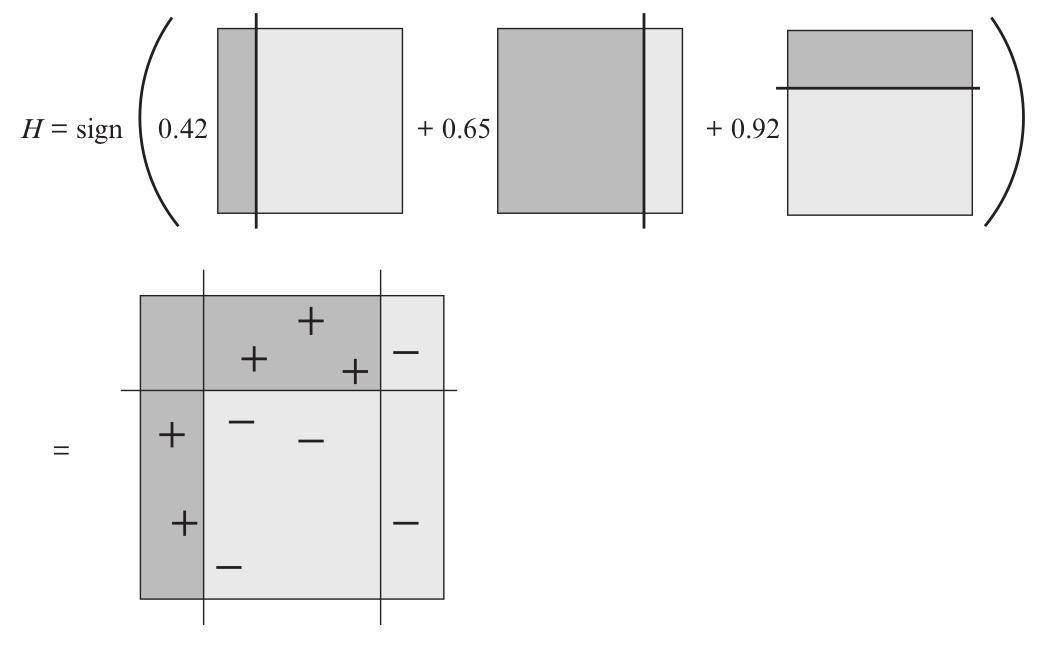
\includegraphics[width=\textwidth]{fig1_2}

figure from \cite{SchapireFreund2014}
}


\frame{\frametitle{AdaBoost: }
\framesubtitle{example}
\centering
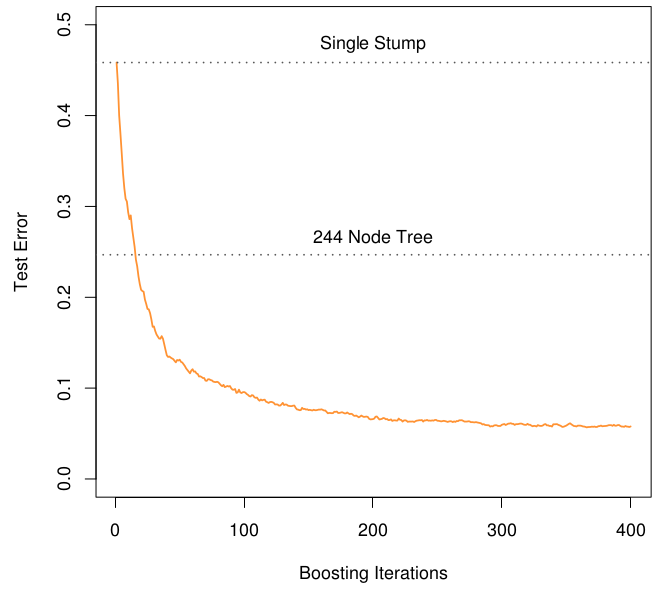
\includegraphics[width=0.8\textwidth]{fig10_2}
}



\section{Statistical Boosting}

\subsection{Boosting as a forward stagewise additive modelling}

\frame{\frametitle{Statistical Boosting: }
\framesubtitle{Boosting as a forward stagewise additive modelling}
The \textcolor{uio}{statistical view} of boosting is based on the concept of {\bf forward stagewise additive modelling}:
\begin{itemize}
\item minimizes a \textcolor{uio}{loss function} $L(y_i, f(x_i))$;
\item using an \textcolor{uio}{additive model},\\
\begin{center} $f(x) = \sum_{m=1}^M \beta_m b(x;\gamma_m)$;\end{center}
\begin{itemize}
\item $b(x;\gamma_m)$ is the \textcolor{uio}{basis}, or \textcolor{uio}{weak learner};
\end{itemize}
\item at \textcolor{uio}{each step},\\
\begin{center} $(\beta_m, \gamma_m) = \text{argmin}_{\beta, \gamma}\sum_{i=1}^N L(y_i, f_{m-1}(x_i)+ \beta b(x_i;\gamma))$;\end{center}
\item the estimate is updated as $f_m(x)=f_{m-1}(x) + \beta_m b(x;\gamma_m)$
\item e.g., in AdaBoost, $\beta_m = \alpha_m/2$, $b(x;\gamma_m)=G(x)$;
\end{itemize}
}

\frame{\frametitle{Statistical Boosting: }
\framesubtitle{Boosting as a forward stagewise additive modelling}
\centering
(see notes)
}

\subsection{Why exponential loss?}

\frame{\frametitle{Statistical Boosting: }
\framesubtitle{Why exponential loss?}
The statistical view of boosting:
\begin{itemize}
\item allows to \textcolor{uio}{interpret} the results;
\item by studying the \textcolor{uio}{properties of the exponential loss};
\end{itemize}

\vspace{12pt}

It is easy to show that
$$
f^*(x)=\text{argmin}_{f(x)} E_{Y|X=x}[e^{-Yf(x)}]=\frac{1}{2}\log\frac{Pr(Y=1|x)}{Pr(Y=-1|x)},
$$
i.e.
$$
Pr(Y=1|x)=\frac{1}{1+e^{-2f^*(x)}};
$$
therefore AdaBoost estimates \textcolor{uio}{1/2 the log-odds} of $Pr(Y=1|x)$.
}


\frame{\frametitle{Statistical Boosting: }
\framesubtitle{Why exponential loss?}
Note:
\begin{itemize}
\item the exponential loss is \textcolor{uio}{not} the only possible loss-function;
\item deviance (cross/entropy): \textcolor{uio}{binomial negative log-likelihood},
$$
-\ell(\pi_x)=-y'\log(\pi_x) - (1-y')\log(1-\pi_x),
$$
where:
\begin{itemize}
\item $y'=(y+1)/2$, i.e., $y'\in \{0,1\}$;
\item $\pi_x = \text{Pr}(Y=1|X=x) = \frac{e^{f(x)}}{e^{-f(x)}+e^{f(x)}} = \frac{1}{1+e^{-2f(x)}}$;
\end{itemize}
\item equivalently,
$$
-\ell(\pi_x)=\log(1+e^{-2yf(x)}).
$$
\item same population minimizers for $E[-\ell(\pi_x)]$ and $E[e^{-Yf(x)}]$.
\end{itemize}
}


\frame{\frametitle{Statistical Boosting: }
\framesubtitle{Why exponential loss?}
\centering
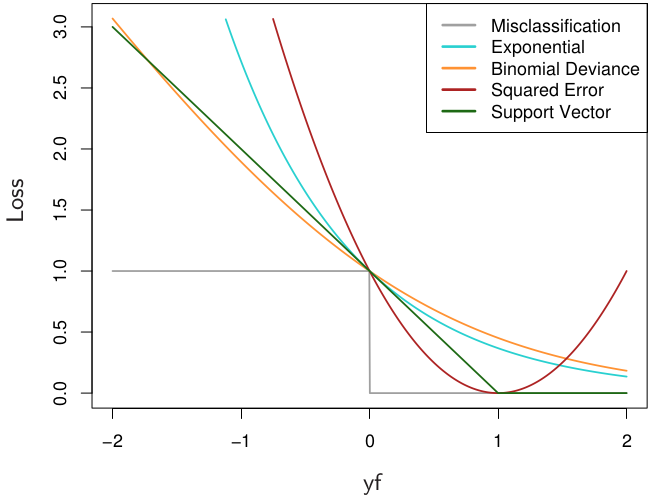
\includegraphics[width=0.92\textwidth]{fig10_4}
}



\subsection{Gradient boosting}

\frame{\frametitle{Statistical Boosting: }
\framesubtitle{Gradient boosting}
We saw that AdaBoost iteratively \textcolor{uio}{minimizes a loss function}.

\vspace{12pt}

In general, consider
\begin{itemize}
\item $L(f) = \sum_{i=1}^N L(y_i, f(x_i))$;
\item $\hat{f} = \text{argmin}_f L(f)$;
\item the \textcolor{uio}{minimization problem} can be solved by considering
$$
f_{m_\text{stop}} = \sum_{m=0}^{m_\text{stop}} h_m
$$
where:
\begin{itemize}
\item $f_0 = h_0$ is the \textcolor{uio}{initial guess};
\item each $f_m$ \textcolor{uio}{improves} the previous $f_{m-1}$ though $h_m$;
\item $h_m$ is called ``\textcolor{uio}{step}''.
\end{itemize}
\end{itemize}
}

\frame{\frametitle{Statistical Boosting: }
\framesubtitle{steepest descent}
The \textcolor{uio}{steepest descent} chooses
$$
h_m = -\rho_m g_m
$$
where
\begin{itemize}
\item $g_m \in \mathds{R}^N$ is the \textcolor{uio}{gradient descent} of $L(f)$ evaluated at $f=f_{m-1}$ and represents the \textcolor{uio}{direction} for the minimization,
$$
g_{im} = \left. \frac{\partial L(y_i, f(x_i))}{\partial f(x_i)}\right|_{f(x_i)=f_{m-1}(x_i)}
$$
\item $\rho_m$ is a scalar and tells ``\textcolor{uio}{how much}'' to minimize
$$
\rho_m = \text{argmin}_\rho L(f_{m-1} - \rho g_m).
$$
\end{itemize}
}

\frame{\frametitle{Statistical Boosting: }
\framesubtitle{example}
Consider the linear Gaussian regression case:
\begin{itemize}
\item $L(y,f(x)) = \frac{1}{2}\sum_{i=1}^N (y_i - f(x_i))^2$;
\item $f(x) = X^T\beta$;
\item initial guess: $\beta \equiv 0$.
\end{itemize}

\vspace{12pt}

Therefore:
\begin{itemize}
\item $g = \frac{\partial \frac{1}{2}\sum_{i=1}^N (y_i - f(x_i))^2}{\partial f(x_i)} = -(y-X^T\beta)$;
\item $g_m = -\left.(y-X^T\beta)\right|_{\beta=0} = -y$;
\item $\rho_m = \text{argmin}_\rho \frac{1}{2}(y - \rho y)^2 \rightarrow \rho_m = X(X^TX)^{-1}X^T$.
\end{itemize}

\vspace{12pt}

Note:
\begin{itemize}
\item overfitting!
\end{itemize}
}


\frame{\frametitle{Statistical Boosting: }
\framesubtitle{shrinkage}
To \textcolor{uio}{regularize} the procedure, a \textcolor{uio}{shrinkage factor} is introduced,
$$
f_m(x) = f_{m-1}(x) + \nu h_m
$$
where $0< \nu < 1$.

\vspace{12pt}

Moreover, $h_m$ can be a \textcolor{uio}{general weak learner} (\textcolor{uio}{base learner}):
\begin{itemize}
\item stump;
\item spline;
\item \dots
\item the idea is to \textcolor{uio}{fit the base learner to the gradient descent} to iteratively minimize the loss function.
\end{itemize}
}


\frame{\frametitle{Statistical Boosting: }
\framesubtitle{Gradient boosting}
{\bf \uline{Gradient boosting algorithm}:}
\begin{enumerate}
\setlength\itemsep{5pt}
\item initialize the estimate, e.g., $f_0(x) = 0$;
\item for $m = 1, \dots, m_\text{stop}$,
\begin{itemize}
\setlength\itemsep{5pt}
  \item[2.1] compute the \textcolor{uio}{negative gradient} vector, $u_m=-\left.\frac{\partial L(y,f(x))}{\partial f(x)}\right|_{f(x)=\hat{f}_{m-1}(x)}$;
  \item[2.2] fit the \textcolor{uio}{base learner} to the negative gradient vector, $h_m(u_m,x)$;
  \item[2.3] \textcolor{uio}{update} the estimate, $f_m(x) = f_{m-1}(x) + \nu h_m(u_m,x)$.
\end{itemize}
\item final estimate, $\hat{f}_{m_\text{stop}}(x) = \sum_{m=1}^{m_\text{stop}} \nu h_m(u_m,x)$
\end{enumerate}

\vspace{12pt}

Note:
\begin{itemize}
 \item $u_m = - g_m$
 \item $\hat{f}_{m_\text{stop}}(x)$ is a \textcolor{uio}{GAM}.
\end{itemize} 
}


\frame{\frametitle{Statistical Boosting: }
\framesubtitle{example}
Consider again the linear Gaussian regression case:
\begin{itemize}
\item $L(y,f(X)) = \frac{1}{2}\sum_{i=1}^N (y_i - f(x_i,\beta))^2$, $f(x_i,\beta) = x_i\beta$;
\item $h(y,X) = X(X^TX)^{-1}X^Ty$.
\end{itemize}

\vspace{4pt}

Therefore:
\begin{itemize}
\item initialize the estimate, e.g., $\hat{f}_0(X, \beta) = 0$;
\item $m = 1$,
\begin{itemize}
  \item $u_1 = -\left.\frac{\partial L(y,f(X,\beta))}{\partial f(X,\beta)}\right|_{f(X,\beta)=\hat{f}_0(X,\beta)} = (y - 0) = y$;
  \item $h_1(u_1,X) = X(X^TX)^{-1}X^Ty$;
  \item $\hat{f}_1(x) = 0 + \nu X(X^TX)^{-1}X^Ty$.
  \item[]
\end{itemize}
\item $m = 2$,
\begin{itemize}
  \item $u_2=-\left.\frac{\partial L(y,f(X,\beta))}{\partial f(X,\beta)}\right|_{f(X,\beta)=\hat{f}_1(X,\beta)} = (y - X^T(\nu\hat{\beta}))$;
  \item $h_2(u_2,X) = X(X^TX)^{-1}X^T(y-X^T(\nu\hat{\beta}))$;
  \item update the estimate, $\hat{f}_2(X,\beta) = \nu X(X^TX)^{-1}X^Ty + \nu X(X^TX)^{-1}X^T(y -X^T(\nu\hat{\beta}))$.
\end{itemize}
\end{itemize}
}


\frame{\frametitle{Statistical Boosting: }
\framesubtitle{remarks}
Note that:
\begin{itemize}
\item we do \textcolor{uio}{not} need to have a linear effects,
\begin{itemize}
 \item $h(y,X)$ can be, e.g., a \textcolor{uio}{spline};
 \end{itemize}
\item using $f(X,\beta) = X^T\beta$, it makes more sense to \textcolor{uio}{work with $\beta$}:
\begin{enumerate}
\setlength\itemsep{5pt}
\item initialize the estimate, e.g., $\hat{\beta}_0 = 0$;
\item for $m = 1, \dots, m_\text{stop}$,
\begin{itemize}
\setlength\itemsep{5pt}
  \item[2.1] compute the negative gradient vector, $u_m=-\left.\frac{\partial L(y,f(X,\beta))}{\partial f(X,\beta)}\right|_{\beta=\hat{\beta}_{m-1}}$;
  \item[2.2] fit the base learner to the negative gradient vector, $b_m(u_m,X) = (X^TX)^{-1}X^Tu_m$;
  \item[2.3] update the estimate, $\hat{\beta}_m = \hat{\beta}_{m-1} + \nu b_m(u_m,x)$.
\end{itemize}
\item final estimate, $\hat{f}_{m_\text{stop}}(x) = X^T\hat{\beta}_m$.
\end{enumerate}
\end{itemize}
}

\frame{\frametitle{Statistical Boosting: }
\framesubtitle{remarks}
Further remarks:
\begin{itemize}
\item for $m_\text{stop} \rightarrow \infty$, $\hat{\beta}_{m_\text{stop}} \rightarrow \hat{\beta}_{OLS}$;
\item the \textcolor{uio}{shrinkage} is controlled by \textcolor{uio}{both $m_\text{stop}$ and $\nu$};
\item usually \textcolor{uio}{$\nu$ is fixed}, $\nu = 0.1$
\item $m_\text{stop}$ is computed by \textcolor{uio}{cross-validation}:
\begin{itemize}
\item it controls the \textcolor{uio}{model complexity};
\item we need an \textcolor{uio}{early stop} to avoid overfitting;
\item if it is \textcolor{uio}{too small} $\rightarrow$ \textcolor{uio}{too much bias};
\item if it is \textcolor{uio}{too large} $\rightarrow$ \textcolor{uio}{too much variance};
\end{itemize}
\item[]
\item the predictors must be \textcolor{uio}{centred}, $E[X_j]=0$.
\end{itemize}
}




%%%%%%%%%%%
\section*{Bibliography}
%%%%%%%%%%%

\frame[allowframebreaks]{\frametitle{References}
\footnotesize
\bibliographystyle{../../../../support/biometrika}
\bibliography{../../../../support/biblio}
}

\end{document}
